\documentclass[a4paper,12pt,french]{article}

\usepackage[cours]{../../Style}

\renewcommand{\arraystretch}{1.3}

\pagestyle{empty}

\geometry{margin=12mm}

% Début du document
%%%%%%%%%%%%%%%%%%%
\begin{document}
\setcounter{section}{1}

\section{Espérance d'une variable aléatoire}

\begin{defin}
\compo
{
On se donne une variable aléatoire $X$ dont la loi est représentée ci-contre.

L'espérance de $X$, notée $\Esp(X)$, est le réel $$\Esp(X):=p_1 x_1 + p_2 x_2 + \ldots + p_N x_N$$
}
{
\begin{center}
\begin{tabularx}{0.9\linewidth}{|c|Y|Y|Y|Y|} \hline
$x$ & $x_1$ & $x_2$ & \ldots & $x_N$ \\ \hline
$\Pro(X=x)$ & $p_1$ & $p_2$ & \ldots & $p_N$ \\ \hline
\end{tabularx}
\end{center}
}
\end{defin}

\begin{rmq}
Celle-ci représente la moyenne des valeurs de $X$ lorsque l'on répète l'expérience aléatoire un très grand nombre de fois.
\end{rmq}

\begin{ex}
On reprend l'exemple ci-dessus. On a $\begin{aligned}[t] \Esp(X) & =0,25 \times (-2) + 0,5 \times 1 + 0,25 \times 4 \\ & = -0,5 + 0,5 + 1 \\ & = 1 \end{aligned}$

L'espérance de $X$ est positive, ce qui veut dire qu'en jouant un grand nombre de fois, le gain moyen par partie sera de 1\euro{} ! Le joueur a donc tout intérêt à faire des parties puisque le jeu est à son avantage.

Évidemment, le jeu restant aléatoire, il est possible (mais très improbable) que le joueur perde dix, cent ou mille parties à la suite et se retrouve ruiné...
\end{ex}

\section{Expériences à plusieurs épreuves: Cas général}

\begin{fait}
Jusqu'à maintenant, on a répété plusieurs expériences régies par une loi équiprobable. On s'intéresse maintenant à des expériences où chaque issue n'a pas forcément la même probabilité.
\end{fait}

\begin{defins}
\begin{itemize}
\item Deux évènements sont dits indépendants si la réalisation de l'un n'a aucune influence sur l'autre.
\item Deux variables aléatoires sont indépendantes si la valeur d'une n'influe pas sur l'autre.
\end{itemize}
\end{defins}

\begin{ex}
\compo[0.6]
{
On dispose de deux urnes contenant chacune dix boules.
\begin{itemize}
\item La première contient quatre boules rouges (R), trois boules jaunes (J) et trois boules bleues (B).
\item La seconde contient six boules vertes (V) et quatre boules noires (N).
\end{itemize}
Par exemple, la probabilité de tirer une boule rouge dans la première urne est $\frac 4 {10}=0,4$.

On tire \textbf{successivement} une boule de la première puis de la seconde urne.

On représente les issues possibles grâce à l'arbre ci-contre.
}
{
\vspace{-7mm}
\begin{center}
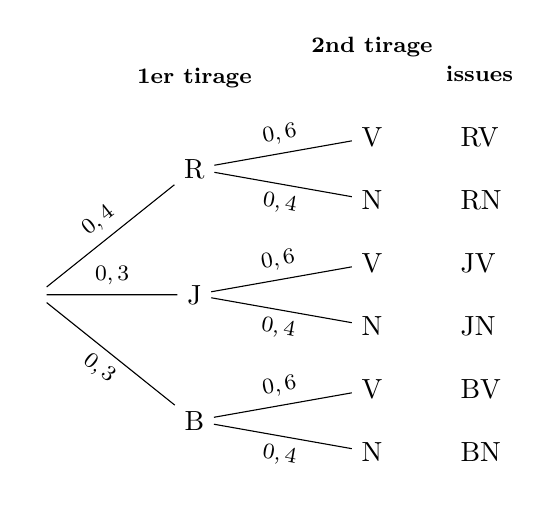
\begin{tikzpicture}[x=2cm,y=0.8cm,legende/.style={midway,sloped,font=\footnotesize}] % Même effet que xscale=1.8 mais l'option sloped marche

\node (O) at (0,0) {};
\node (R) at (1,2) {R};
\node (J) at (1,0) {J};
\node (B) at (1,-2) {B};
\node[anchor=west] (RV) at (2,2.5) {V};
\node[anchor=west] (RN) at (2,1.5) {N};
\node[anchor=west] (JV) at (2,0.5) {V};
\node[anchor=west] (JN) at (2,-0.5) {N};
\node[anchor=west] (BV) at (2,-1.5) {V};
\node[anchor=west] (BN) at (2,-2.5) {N};

\node[right of=RV,anchor=west,node distance=1cm] (res) {RV};
\node[right of=RN,anchor=west,node distance=1cm] {RN};
\node[right of=JV,anchor=west,node distance=1cm] {JV};
\node[right of=JN,anchor=west,node distance=1cm] {JN};
\node[right of=BV,anchor=west,node distance=1cm] {BV};
\node[right of=BN,anchor=west,node distance=1cm] {BN};

\node[font=\footnotesize\bfseries,above of=R,node distance=1.15cm] (lancer1) {1\up{er} tirage};
\node[font=\footnotesize\bfseries,above of=RV,node distance=1.15cm] (lancer2) {2\up{nd} tirage};
\node[font=\footnotesize\bfseries,above of=res,node distance=0.8cm] {issues};

%\draw[->] (lancer1) -- (P);
%\draw[->] (lancer2) -- (PP);

\draw (O) -- (R) node[legende,above] {$0,4$} (R) -- (RV) node[legende,above] {$0,6$} (R) -- (RN) node[legende,below] {$0,4$} (O) -- (J) node[legende,above] {$0,3$} (J) -- (JV) node[legende,above] {$0,6$} (J) -- (JN) node[legende,below] {$0,4$} (O) -- (B) node[legende,below] {$0,3$} (B) -- (BV) node[legende,above] {$0,6$} (B) -- (BN) node[legende,below] {$0,4$};
\end{tikzpicture}
\end{center}
}

\end{ex}

\newpage

\begin{proprs}
Pour construire et utiliser un arbre de probabilités, on utilisera les règles suivantes:
\begin{itemize}
\item La somme des probabilités inscrites sur les branches issues d'un même noeud est égale à 1;
\item La probabilité d'une issue représentée par un chemin est \textbf{le produit} des probabilités inscrite sur chacune de ses branches;
\item La probabilité d'un évènement est la somme des probabilité de tous les chemins menant à cet évènement.
\end{itemize}
\end{proprs}

\begin{exs}
\compo[0.55]
{
\begin{itemize}
\item La probabilité d'obtenir une boule rouge puis une boule verte {\color{DarkRed}(RV)} est: $$0,4 \times 0,6 = 0,54$$
\item La probabilité d'obtenir une boule autre que rouge puis une boule noire {\color{DarkBlue}(JN ou BN)} est:
$$\begin{aligned} (0,3 \times 0,6) + (0,3 \times 0,6) & = 0,18 + 0,18 \\ & = 0,36 \end{aligned}$$
\end{itemize}
}
{
\vspace{-7mm}
\begin{center}
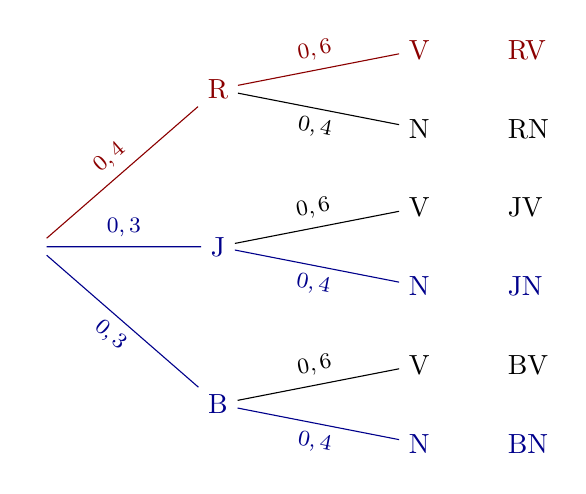
\begin{tikzpicture}[x=2.3cm,legende/.style={midway,sloped,font=\footnotesize}] % Même effet que xscale=1.8 mais l'option sloped marche

\node (O) at (0,0) {};
\node[DarkRed] (R) at (1,2) {R};
\node[DarkBlue] (J) at (1,0) {J};
\node[DarkBlue] (B) at (1,-2) {B};
\node[anchor=west,DarkRed] (RV) at (2,2.5) {V};
\node[anchor=west] (RN) at (2,1.5) {N};
\node[anchor=west] (JV) at (2,0.5) {V};
\node[anchor=west,DarkBlue] (JN) at (2,-0.5) {N};
\node[anchor=west] (BV) at (2,-1.5) {V};
\node[anchor=west,DarkBlue] (BN) at (2,-2.5) {N};

\node[right of=RV,anchor=west,node distance=1cm,DarkRed] (res) {RV};
\node[right of=RN,anchor=west,node distance=1cm] {RN};
\node[right of=JV,anchor=west,node distance=1cm] {JV};
\node[right of=JN,anchor=west,node distance=1cm,DarkBlue] {JN};
\node[right of=BV,anchor=west,node distance=1cm] {BV};
\node[right of=BN,anchor=west,node distance=1cm,DarkBlue] {BN};

%\node[font=\footnotesize\bfseries,above of=R,node distance=1.05cm] (lancer1) {1\up{ère} tirage};
%\node[font=\footnotesize\bfseries,above of=RV,node distance=1.15cm] (lancer2) {2\up{nd} tirage};
%\node[font=\footnotesize\bfseries,above of=res,node distance=0.7cm] {issues};

%\draw[->] (lancer1) -- (P);
%\draw[->] (lancer2) -- (PP);

\draw[DarkRed] (O) -- (R) node[legende,above] {$0,4$} (R) -- (RV) node[legende,above] {$0,6$};

\draw[DarkBlue] (O) -- (J) node[legende,above] {$0,3$} (J) -- (JN) node[legende,below] {$0,4$} (O) -- (B) node[legende,below] {$0,3$}(B)  -- (BN) node[legende,below] {$0,4$};

\draw (R) -- (RN) node[legende,below] {$0,4$} (J) -- (JV) node[legende,above] {$0,6$} (B) -- (BV) node[legende,above] {$0,6$};
\end{tikzpicture}
\end{center}
}
\end{exs}

\vfill

\begin{proprs}
Pour construire et utiliser un arbre de probabilités, on utilisera les règles suivantes:
\begin{itemize}
\item La somme des probabilités inscrites sur les branches issues d'un même noeud est égale à 1;
\item La probabilité d'une issue représentée par un chemin est \textbf{le produit} des probabilités inscrite sur chacune de ses branches;
\item La probabilité d'un évènement est la somme des probabilité de tous les chemins menant à cet évènement.
\end{itemize}
\end{proprs}

\begin{exs}
\compo[0.55]
{
\begin{itemize}
\item La probabilité d'obtenir une boule rouge puis une boule verte {\color{DarkRed}(RV)} est: $$0,4 \times 0,6 = 0,54$$
\item La probabilité d'obtenir une boule autre que rouge puis une boule noire {\color{DarkBlue}(JN ou BN)} est:
$$\begin{aligned} (0,3 \times 0,6) + (0,3 \times 0,6) & = 0,18 + 0,18 \\ & = 0,36 \end{aligned}$$
\end{itemize}
}
{
\vspace{-7mm}
\begin{center}
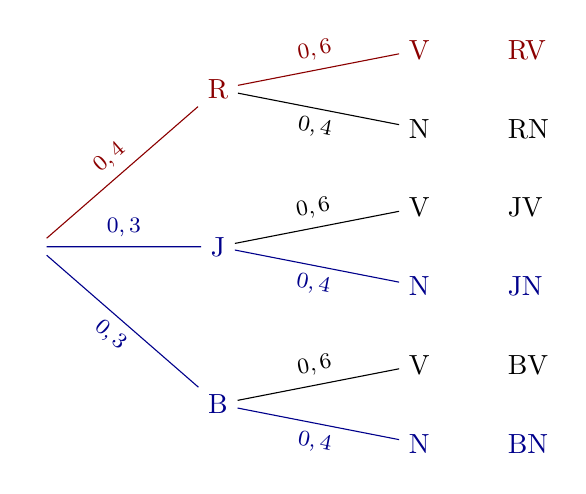
\begin{tikzpicture}[x=2.3cm,legende/.style={midway,sloped,font=\footnotesize}] % Même effet que xscale=1.8 mais l'option sloped marche

\node (O) at (0,0) {};
\node[DarkRed] (R) at (1,2) {R};
\node[DarkBlue] (J) at (1,0) {J};
\node[DarkBlue] (B) at (1,-2) {B};
\node[anchor=west,DarkRed] (RV) at (2,2.5) {V};
\node[anchor=west] (RN) at (2,1.5) {N};
\node[anchor=west] (JV) at (2,0.5) {V};
\node[anchor=west,DarkBlue] (JN) at (2,-0.5) {N};
\node[anchor=west] (BV) at (2,-1.5) {V};
\node[anchor=west,DarkBlue] (BN) at (2,-2.5) {N};

\node[right of=RV,anchor=west,node distance=1cm,DarkRed] (res) {RV};
\node[right of=RN,anchor=west,node distance=1cm] {RN};
\node[right of=JV,anchor=west,node distance=1cm] {JV};
\node[right of=JN,anchor=west,node distance=1cm,DarkBlue] {JN};
\node[right of=BV,anchor=west,node distance=1cm] {BV};
\node[right of=BN,anchor=west,node distance=1cm,DarkBlue] {BN};

%\node[font=\footnotesize\bfseries,above of=R,node distance=1.05cm] (lancer1) {1\up{ère} tirage};
%\node[font=\footnotesize\bfseries,above of=RV,node distance=1.15cm] (lancer2) {2\up{nd} tirage};
%\node[font=\footnotesize\bfseries,above of=res,node distance=0.7cm] {issues};

%\draw[->] (lancer1) -- (P);
%\draw[->] (lancer2) -- (PP);

\draw[DarkRed] (O) -- (R) node[legende,above] {$0,4$} (R) -- (RV) node[legende,above] {$0,6$};

\draw[DarkBlue] (O) -- (J) node[legende,above] {$0,3$} (J) -- (JN) node[legende,below] {$0,4$} (O) -- (B) node[legende,below] {$0,3$}(B)  -- (BN) node[legende,below] {$0,4$};

\draw (R) -- (RN) node[legende,below] {$0,4$} (J) -- (JV) node[legende,above] {$0,6$} (B) -- (BV) node[legende,above] {$0,6$};
\end{tikzpicture}
\end{center}
}
\end{exs}

\end{document}
